
Find the smaller area enclosed by the circle  $\vec{x}\vec{x}^T=4$ and the line $\myvec{1 & 1} \vec{x}=2$.
General equation of circle is 
\begin{align}
{\vec{x}^T\vec{x}} + 2\vec{u}^T\vec{x} + f = 0 \label{eq:solutions/1/11/eq1}\\
 \norm{\vec{x}}^2 + 2\vec{u}_1^T\vec{x} + f_1 = 0\label{eq:solutions/1/11/eq2}\\
 {\vec{x}^{T}\vec{x}}-4=0 \label{eq:solutions/1/11/eq3}\\
 \vec{u_1}=\myvec{0\\0}\label{eq:solutions/1/11/eq4}\\
 f_1=-4\label{eq:solutions/1/11/eq5}\\
\vec{O_1}=\myvec{0\\0}\label{eq:solutions/1/11/eq6}\\
r=\sqrt{\vec{c}^{T}\vec{c}-f} = \sqrt{4}\label{eq:solutions/1/11/eq7}\\
    \implies \boxed{r=2} \label{eq:solutions/1/11/eq8}
 \end{align}
From equation \eqref{eq:solutions/1/11/eq8}, the point at which circle touches $x$-axis is \myvec{-2\\0} and \myvec{2\\0}.\\
The direction vector of the given line $\myvec{1&1}\vec{x}=2$ is $\myvec{-1\\1}$.\\

\begin{figure}[!ht]
	\centering
	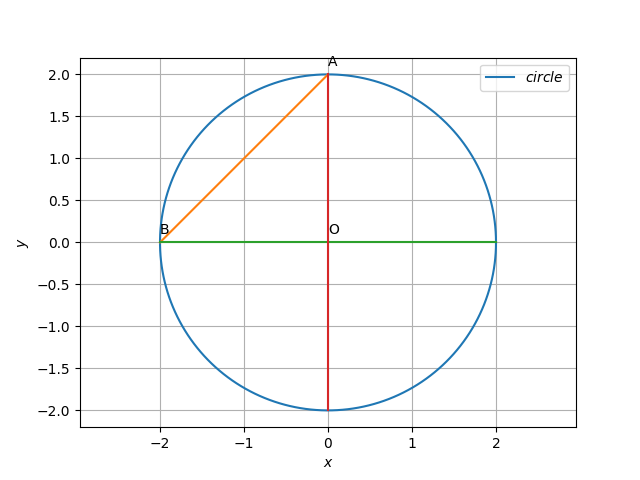
\includegraphics[width=\columnwidth]{./solutions/conics/1/11/circle.png}
	\caption{Smaller area enclosed by line and circle}
	\label{eq:solutions/1/11/eq:myfig}
\end{figure}

To find point $\vec{A}$ and $\vec{B}$,
The parametric form of line is,
\begin{align}
    \vec{A} = \vec{q}+\lambda\vec{m}\label{eq:solutions/1/11/eq9}\\
            = \myvec{1\\1}+\lambda\myvec{-1\\1}\label{eq:solutions/1/11/eq10}\\
    \lambda^2 = \frac{-f_1-\norm{\vec{q}}^2}{\norm{\vec{m}}^2}\label{eq:solutions/1/11/eq11}\\
                = \frac{4-2}{2} = 1\label{eq:solutions/1/11/eq12}\\
    \implies \lambda = \pm{1} \label{eq:solutions/1/11/eq13}\\
    \vec{A} = \myvec{0\\2}\quad \vec{B} = \myvec{-2\\0}\label{eq:solutions/1/11/eq14}\\
    \vec{O} = \myvec{0\\0} \\
    (\vec{A-O}) = \myvec{0\\2}\\
    (\vec{B-O}) = \myvec{-2\\0}
\end{align}
Inner product of $(\vec{A-O})$ and $(\vec{B-O})$ is given as:
\begin{align}
(\vec{A-O})^T(\vec{B-O})=0
\end{align}
Therefore, $(\vec{A-O}) \perp (\vec{B-O})$ \\
Smaller area enclosed by circle and line $\bf{AB}$ is:\\
 Area = (Area of circle in 2nd Quadrant) - (Area of right triangle formed by line AB, X and Y axis)
 \begin{align}
Area=\frac{\pi\theta_1}{360}r^2-\frac{1}{2}\times2\times2\label{eq:solutions/1/11/eq15}\\
=\frac{90}{360}\pi\times2^2-2\label{eq:solutions/1/11/eq16}\\
=\pi-2\label{eq:solutions/1/11/eq17}
\end{align}
Hence, the smaller area enclosed by the circle  $\vec{x}\vec{x}^T=4$ and the line $\myvec{1 & 1} \vec{x}=2$ is $(\pi-2)$
